\documentclass{article}

% \CorrectChoiceEmphasis{\color{red}\bfseries}
\usepackage{amssymb, amsmath, amsfonts}
\usepackage{geometry}
\usepackage{graphicx}
\usepackage{tikz}
\usetikzlibrary{calc}
\usepackage{pgfplots}
\usepackage{multirow,array} % for payoff matrix formatting
\usepackage{hyperref}
\usepackage{xcolor}
\hypersetup{
  colorlinks = true,
  linkcolor  = gray,
  urlcolor   = blue
}

\usepackage{exsheets}
\newcounter{questions}
\SetupExSheets{
  headings = block-wp,
  % solution/print = true % set this to true to print key
}

\usepackage{etoolbox}

% mark mc options as correct with custom \correct command
\newcommand{\ShowAnswers}{false}
% \renewcommand{\ShowAnswers}{true} %comment this out if you do not want to show the answers
\newcommand{\correct}{%
    \expandafter\ifstrequal\expandafter{\ShowAnswers}{true}{\bfseries}{}%
}

\definecolor{crimson}{RGB}{ 170, 4, 36 }
\definecolor{darkblue}{RGB}{ 4, 47, 170 }
\definecolor{brown}{RGB}{ 111, 71, 2 }
\definecolor{periwinkle}{RGB}{ 90, 177, 204 }
\definecolor{ducksgreen}{HTML}{007030}
\definecolor{darkgray}{RGB}{169, 169, 169}
\definecolor{dimgray}{RGB}{105, 105, 105}

\geometry{left=1.0in,right=1.0in,top=1.0in,bottom=1.0in}

% \pagestyle{headandfoot}
% \lhead{EC327 Game Theory}
% \chead{Practice Midterm}
% \rhead{Winter 2024}
% \runningheadrule

\title{
    \textbf{Econ 327: Game Theory} \\ 
    Practice Exam
    }
\author{University of Oregon}
\date{\today}

% exam-type question formatting
% \renewcommand{\thequestion}{\textbf{Question \arabic{question}}}
% \bracketedpoints

\begin{document}

\variant{2}

\maketitle

\begin{center}
  \Large{\textbf{Version 1}}
\end{center}

% \begin{center}
%   \gradetable[h][questions]
% \end{center}

% \vspace{0.5in}

% \begin{center}
%   \textbf{For homework assignments:}
% \end{center}
% 
% \begin{itemize}
% 
% %  \item DO NOT write your name:
% %  this assignment will be graded anonymously. 
% %  If you want to, you can include your student ID instead.
% 
%   \item Complete \textit{all} questions and enumerate.
%   I will select one question at random to be graded
%   according to the rubric on Canvas.
% 
%   \item You may choose to work with others,
%   but everyone must submit to Canvas individually.
%   Please include the names of everyone who you worked with 
%   below your own name.
%  
% \end{itemize}

\begin{center}
  \textbf{For Exams:}
\end{center}

\begin{itemize}
  
  \item Complete \textit{all} questions and enumerate. 
  All questions will be graded.

  \item Carefully explain all your answers on short and long answer questions.

  An incorrect answer with clear explanation will earn partial credit,
  an incorrect answer with no work will get zero points.

  \item 
  If you do not understand what a question is asking for, 
  ask for clarification. 

\end{itemize}

\underline{Allowed Materials:}

\begin{itemize}
 
  \item A single 5" by 3" note card

  \item A non-programmable calculator

  \item Pencils, color pens, eraser, ruler/straight-edge etc.
\end{itemize}

\vspace{1.0in}

\makebox[.6\textwidth]{Name\enspace\hrulefill}

\vspace{0.5in}

\begin{center}
  \fbox{\fbox{\parbox{5.5in}{\centering
    Answer the questions in the spaces provided on the
    question sheets. If you run out of room for an answer,
    continue on the back of the page or another sheet of paper.}}}
\end{center}

\newpage

% \begin{questions}

%------------------------------------------------------------------%

% \begin{question}[20] 

\section*{Multiple Choice}

\begin{question}[ID=1,type=exam]{4}
  For the strategic form game below:
  \begin{table}[!h]
    \begin{center}
    \setlength{\extrarowheight}{2pt}
    \begin{tabular}{*{4}{c|}}
      \multicolumn{2}{c}{} & \multicolumn{2}{c}{$P_2$} \\\cline{3-4}
      \multicolumn{1}{c}{} &      & Left & Right \\\cline{2-4}
      \multirow{2}*{$P_1$} & Up   & 3,3  & 9,4   \\\cline{2-4}
                           & Down & 5,2  & 6,1   \\\cline{2-4}
    \end{tabular}
    \end{center}
  \end{table} \\
  let $p$ be the \textbf{probability Player 1 chooses Up}
  and let $q$ be the probability \textbf{Player 2 chooses Left}.
  Choose the correct Expected Utility expression for Player 1's strategy Up.
  \begin{tasks}
    \task \vary{$3p + 9(1-p)$}{$3q + 4(1-q)$} 
    \task \vary{\correct $3q + 9(1-q)$}{$3p + 9(1-p)$}
    \PrintSolutionsTF{Correct}{}
    \task \vary{$3q + 4(1-q)$}{$3p + 5(1-q)$}
    \task \vary{$3p + 5(1-q)$}{\correct $3q + 9(1-q)$}
    \PrintSolutionsTF{}{Correct}
  \end{tasks}
\end{question}

\begin{question}[ID=2,type=exam]{4}
  For the strategic form game below:
  \begin{table}[!h]
    \begin{center}
    \setlength{\extrarowheight}{2pt}
    \begin{tabular}{*{4}{c|}}
      \multicolumn{2}{c}{} & \multicolumn{2}{c}{$P_2$} \\\cline{3-4}
      \multicolumn{1}{c}{} &      & Close & Far \\\cline{2-4}
      \multirow{2}*{$P_1$} & High & 9,5   & 5,1 \\\cline{2-4}
                           & Low  & 6,2   & 6,8 \\\cline{2-4}
    \end{tabular}
    \end{center}
  \end{table} \\
  let $p$ be the \textbf{probability Player 1 chooses High}
  and let $q$ be the probability \textbf{Player 2 chooses Close}.
  Choose the correct Expected Utility expression for \textbf{Player 2's strategy Close}.
  \begin{tasks}
    \task \vary{\correct $5p + 2(1-p)$}{$1p + 8(1-p)$} \PrintSolutionsTF{Correct}{}
    \task \vary{$1p + 8(1-p)$}{$5q + 1(1-q)$}
    \task \vary{$5q + 1(1-q)$}{$2p + 8(1-q)$}
    \task \vary{$2p + 8(1-q)$}{\correct $5p + 2(1-p)$} \PrintSolutionsTF{}{Correct}
  \end{tasks}
\end{question}

\begin{question}[ID=3,type=exam]{4}
  For the strategic form game below:
  \begin{table}[!h]
    \begin{center}
    \setlength{\extrarowheight}{2pt}
    \begin{tabular}{*{4}{c|}}
      \multicolumn{2}{c}{} & \multicolumn{2}{c}{$P_2$} \\\cline{3-4}
      \multicolumn{1}{c}{} &      & Push & Pull  \\\cline{2-4}
      \multirow{2}*{$P_1$} & Give & 6, 9 & 12, 8 \\\cline{2-4}
                           & Take & 9, 4 & 7 ,10 \\\cline{2-4}
    \end{tabular}
    \end{center}
  \end{table} \\
  Which of the following mixed strategy profiles is a Nash equilibrium?
  \begin{tasks}
    \task \vary{
      \correct $\sigma_1$ = (6/7 Give, 1/7 Take), $\sigma_2$ = (5/8 Push, 3/8 Pull)
    }{
      $\sigma_1$ = (2/5 Give, 3/5 Take), $\sigma_2$ = (1/2 Push, 1/2 Pull)
    }
    \task \vary{
      $\sigma_1$ = (1/2 Give, 1/2 Take), $\sigma_2$ = (1/2 Push, 1/2 Pull)
    }{
      \correct $\sigma_1$ = (6/7 Give, 1/7 Take), $\sigma_2$ = (5/8 Push, 3/8 Pull)
    }
    \task \vary{
      $\sigma_1$ = (1/3 Give, 2/3 Take), $\sigma_2$ = (5/6 Push, 1/6 Pull)
    }{
      $\sigma_1$ = (1/2 Give, 1/2 Take), $\sigma_2$ = (1/2 Push, 1/2 Pull)
    }
    \task \vary{
      $\sigma_1$ = (2/5 Give, 3/5 Take), $\sigma_2$ = (1/2 Push, 1/2 Pull)
    }{
      $\sigma_1$ = (1/3 Give, 2/3 Take), $\sigma_2$ = (5/6 Push, 1/6 Pull)
    }
  \end{tasks}
\end{question}

  \begin{question}[ID=4,type=exam]{4}
  Consider the strategic form game below:
  \begin{table}[h!]
    \begin{center}
    \setlength{\extrarowheight}{2pt}
    \begin{tabular}{*{4}{c|}}
      \multicolumn{2}{c}{} & \multicolumn{2}{c}{$P_2$} \\\cline{3-4}
      \multicolumn{1}{c}{} &    & X   & Y  \\\cline{2-4}
      \multirow{3}*{$P_1$}  & A & 2,3 & 6,1 \\\cline{2-4}
                            & B & 4,2 & 1,3 \\\cline{2-4}
                            & C & 3,1 & 2,4 \\\cline{2-4}
    \end{tabular}
    \end{center}
  \end{table}
  Suppose Player 1 plays A with probability $\alpha$,
  B with probability $\beta$,
  and C with probability $\gamma$.
  When will Player 1 be indifferent between playing X and playing Y?
  \begin{tasks}
    \task \vary{$2\alpha+4\beta+3\gamma=6\alpha+1\beta+2\gamma$}{$3\alpha+1\alpha=2\beta+3\beta=1\gamma+4\gamma$}
    \task \vary{$3\alpha+1\alpha=2\beta+3\beta=1\gamma+4\gamma$}{\correct $3\alpha+2\beta+1\gamma=1\alpha+3\beta+4\gamma$}
    \PrintSolutionsTF{}{Correct}
    \task \vary{\correct $3\alpha+2\beta+1\gamma=1\alpha+3\beta+4\gamma$}{$\alpha=\beta=\gamma$}
    \PrintSolutionsTF{Correct}{}
    \task \vary{$\alpha=\beta=\gamma$}{$2\alpha+4\beta+3\gamma=6\alpha+1\beta+2\gamma$}
  \end{tasks}
\end{question}

  \begin{question}[ID=5,type=exam]{4} 
  A player using a \textbf{mixed strategy} means that:
  \begin{tasks}
    \task \vary
    {some parts of their strategy are played simultaneously and other parts are played sequentially}
    {\correct they are internally uncertain about which action they will choose because they are acting randomly} % correct
    \task \vary
    {they are confused about what action their opponent is taking}
    {some parts of their strategy are played simultaneously and other parts are played sequentially}
    \task \vary
    {\correct they are internally uncertain about which action they will choose because they are acting randomly} % correct
    {they will regret not having chosen their a pure strategy instead}
    \task \vary
    {they will regret not having chosen their a pure strategy instead}
    {they are confused about what action their opponent is taking}
  \end{tasks}
\end{question}

\begin{question}[ID=6,type=exam]{4}
  A game featuring \textbf{asymmetric information}:
  \begin{tasks}
    \task \vary
    {\correct has some players who have access to private information which is not directly observable to others} % correct
    {is repeated multiple times by the same players}
    \task \vary
    {means that one player has a strategy with no equivalent strategy avaibable to any other player}
    {has Nature acting as a player even though she doesn't have any preference over outcomes}
    \task \vary
    {has Nature acting as a player even though she doesn't have any preferences}
    {means that one player has a strategy with no equivalent strategy avaibable to any other player}
    \task \vary
    {is repeated multiple times by the same players}
    {\correct has some players who have access to private information which is not directly observable to others} % correct
  \end{tasks}
\end{question}

\begin{question}[ID=7,type=exam]{4}
  \setlist{nolistsep}
  By \textbf{\vary{screening}{signaling}}:
  \begin{tasks}
    \task \vary
    {\correct a player attempts to learn about some private information held by others by designing an incentive mechanism} % correct
    {only players with the `bad' condition sort into a market}
    \task \vary
    {a player can reveal their own private information through their actions}
    {\correct a player can reveal their own private information through their actions} % correct
    \task \vary
    {only players with the `bad' condition sort into a market}
    {a player can reveal the private information held by others by designing an incentive mechanism}
    \task \vary
    {only mixed strategies will be played in equilibrium}
    {only mixed strategies will be played in equilibrium}
  \end{tasks}
\end{question}

\begin{question}[ID=8,type=exam]{4}
  Consider the strategic form game below:
  \begin{table}[h!]
    \begin{center}
    \begin{tabular}{*{5}{c|}}
      \multicolumn{2}{c}{} & \multicolumn{3}{c}{$P_2$} \\\cline{3-5}
      \multicolumn{1}{c}{} &         & Left & Middle & Right \\\cline{2-5}
      \multirow{3}*{$P_1$}& Up       & 0,1  & 9,0    & 2,3 \\\cline{2-5}
                          & Straight & 5,9  & 7,3    & 1,7 \\\cline{2-5}
                          & Down     & 7,5  & 10,10  & 3,5 \\\cline{2-5}
    \end{tabular}
    \end{center}
  \end{table} \\
  How many Nash equilibria exist in this simultaneous game,
  including both \textbf{pure} and \textbf{mixed} strategies?
  \begin{tasks}
    \task \correct One equilibrium
    \task Two equilibria
    \task Three equilibria
    \task An infinite number of equilibria
  \end{tasks}
\end{question}

\begin{question}[ID=9,type=exam]{4}
  An \textbf{information set}:
  \begin{tasks}
    \task \vary
    {is used by game theorists to signal how they want their games to be played}
    {holds all pieces of information which are publically observable to all players}
    \task \vary
    {tells a player what action to take}
    {is used by game theorists to signal how they want their games to be played}
    \task \vary
    {\correct contains all decision nodes which a player cannot tell the difference between when they reach that part of the game} % correct
    {tells a player what action to take}
    \task \vary
    {holds all pieces of information which are publically observable to all players}
    {\correct contains all decision nodes which a player cannot tell the difference between when they reach that part of the game} % correct
  \end{tasks}
\end{question}

\begin{question}[ID=10,type=exam]{4}
  Consider the following lottery: \\
  \begin{itemize}
    \item with probability \vary{1/4}{1/2} you will receive \$1,600.
    \item with probability \vary{3/4}{1/2} you only receive \$16.
  \end{itemize}
  Suppose someone has a risk-averse utility function of $u(\$x) = \sqrt{\$x}$.
  For what certain amount of dollars, $x$, will this person be indifferent
  between taking the certain payment with probability of 1
  and taking the lottery defined above?
  \begin{tasks}
    \task \vary{\correct \$169}{\$169}
    \task \vary{\$412}{\correct \$412}
    \task \vary{\$484}{\$484}
    \task \vary{\$808}{\$808}
  \end{tasks}
\end{question}


\begin{question}[ID=11,type=exam]{4}
  Identify the class concept that most closely describes the situation below: \\
  Conspicuous consumption describes the phenomenon of buying flashy luxury goods with visible branding
  such as Louis Vuitton, Gucci, Prada, etc.
  in order to display the buyer's level of wealth to be able to afford such goods.
  \begin{tasks}
    \task \vary
    {Brinksmanship}{Risk sharing}
    \task \vary
    {Mixed Strategy Nash Equilibrium}{\correct Signaling}
    \task \vary
    {Risk sharing}{Brinksmanship}
    \task \vary
    {\correct Signaling}{Mixed Strategy Nash Equilibrium}
  \end{tasks}
\end{question}

\begin{question}[ID=12,type=exam]{4}
  In the \textbf{Prisoner’s Dilemma}, mutual cooperation:
  \begin{tasks}
    \task \vary
    {is a dominant strategy equilibrium}
    {\correct Pareto dominates the outcome of mutual defection}
    \task \vary
    {\correct Pareto dominates the outcome of mutual defection}
    {is stable}
    \task \vary
    {is stable}
    {is a credible threat}
    \task \vary
    {is a credible threat}
    {is a dominant strategy equilibrium}
  \end{tasks}
\end{question}

\begin{question}[ID=13,type=exam]{4}
  The Folk Theorem states that:
  \begin{tasks}
    \task \vary{\correct Any individually rational and feasible outcome can be reached in a repeated game for some sufficiently high enough discount factor.}{The Prisoners' Dilemma is the only game with a unique Nash equilibrium.}
    \task \vary{All Pareto optimal outcomes can always be reached in a Nash equilibrium.}{\correct Any individually rational and feasible outcome can be reached in a repeated game for some sufficiently high enough discount factor.}
    \task \vary{No matter how hard you try, some folks will just never cooperate}{All Pareto optimal outcomes can always be reached in a Nash equilibrium.}
    \task \vary{The Prisoners' Dilemma is the only game with a unique Nash equilibrium.}{No matter how hard you try, some folks will just never cooperate}
  \end{tasks}
\end{question}

\begin{question}[ID=14,type=exam]{4}
  Consider the Prisoners' Dilemma game with payoffs as shown in the strategic form table below: \\
  \begin{table}[!h]
    \begin{center}
    \setlength{\extrarowheight}{2pt}
    \begin{tabular}{*{4}{c|}}
      \multicolumn{2}{c}{} & \multicolumn{2}{c}{$P_2$} \\\cline{3-4}
      \multicolumn{1}{c}{} &           & Cooperate         & Cheat \\\cline{2-4}
      \multirow{2}*{$P_1$} & Cooperate & \vary{5, 5}{6, 6} & \vary{-7,9}{-6,10}\\\cline{2-4}
                           &     Cheat & \vary{9,-7}{10,-6} & \vary{0, 0}{0, 0}\\\cline{2-4}
    \end{tabular}
    \end{center}
  \end{table} \\
  Suppose Player 2 is utilizing a 
    \textbf{Tit-for-Tat} strategy in which they will start off cooperating,
    and after that they will play whatever strategy their oponent used in the previous round. \\
    Which of the following represents Player 1's present value
    of cheating in the first period and then going cooperating in all following periods?
  \begin{tasks}
    \task \vary
    {$9 + 0\delta + 0\delta^2 + 0\delta^3 + ... = 9$}
    {$10 + 0\delta + 0\delta^2 + 0\delta^3 + ... = 10$}
    \task \vary
    {$5 + 5\delta + 5\delta^2 + 5\delta^3 + ... = \frac{5}{1-\delta}$}
    {$6 + 6\delta + 6\delta^2 + 6\delta^3 + ... = \frac{6}{1-\delta}$}
    \task \vary
    {$9 + 5\delta + 5\delta^2 + 5\delta^3 + ... = 9 + 5\frac{\delta}{1-\delta}$}
    {$10 + 6\delta + 6\delta^2 + 6\delta^3 + ... = 10 + 6\frac{\delta}{1-\delta}$}
    \task \vary
    {\correct $9 - 7\delta + 5\delta^2 + 5\delta^3 + ... = 9 - 7\delta + 5\frac{\delta^2}{1-\delta}$}
    {\correct $10 - 6\delta + 6\delta^2 + 6\delta^3 + ... = 10 - 6\delta + 6\frac{\delta^2}{1-\delta}$}
    \PrintSolutionsTF{Correct}{}
  \end{tasks}
\end{question}

\begin{question}[ID=15,type=exam]{4}
  Consider the Prisoners' Dilemma game with payoffs as shown in the strategic form table below: \\
  \begin{table}[!h]
    \begin{center}
    \setlength{\extrarowheight}{2pt}
    \begin{tabular}{*{4}{c|}}
      \multicolumn{2}{c}{} & \multicolumn{2}{c}{$P_2$} \\\cline{3-4}
      \multicolumn{1}{c}{} &           & Cooperate         & Cheat \\\cline{2-4}
      \multirow{2}*{$P_1$} & Cooperate & \vary{8, 8}{9, 9} & \vary{2,10}{5,15}\\\cline{2-4}
                           &     Cheat & \vary{10,2}{15,5} & \vary{4, 4}{7, 7}\\\cline{2-4}
    \end{tabular}
    \end{center}
  \end{table} \\
  Suppose Player 2 is utilizing a 
    \textbf{Grim Trigger} strategy in which they will start off cooperating,
    and continue to cooperate unless their opponent has ever played Cheat,
    in which case they will play Cheat in all periods following. \\
    Which of the following represents Player 1's present value
    of cheating in the first period (and in all following periods)?
    $\delta$ is the per-period discount rate.
  \begin{tasks}
    \task \vary
    {\correct $10 + 4\delta + 4\delta^2 + 4\delta^3 + ... = 10 + 4\frac{\delta}{1-\delta}$}
    {\correct $15 + 7\delta + 7\delta^2 + 7\delta^3 + ... = 15 + 7\frac{\delta}{1-\delta}$}
    \PrintSolutionsTF{Correct}{}
    \task \vary
    {$8 + 8\delta + 8\delta^2 + 8\delta^3 + ... = \frac{8}{1-\delta}$}
    {$9 + 9\delta + 9\delta^2 + 9\delta^3 + ... = \frac{9}{1-\delta}$}
    \task \vary
    {$10 + 8\delta + 8\delta^2 + 8\delta^3 + ... = 10 + 8\frac{\delta}{1-\delta}$}
    {$15 + 9\delta + 9\delta^2 + 9\delta^3 + ... = 15 + 9\frac{\delta}{1-\delta}$}
    \task \vary
    {$10 + 2\delta + 8\delta^2 + 8\delta^3 + ... = 10 + 2\delta + 8\frac{\delta^2}{1-\delta}$}
    {$15 + 5\delta + 9\delta^2 + 9\delta^3 + ... = 15 + 5\delta + 9\frac{\delta^2}{1-\delta}$}
  \end{tasks}
\end{question}


\noindent\fbox{
  \parbox{\linewidth}{
  See the Canvas quizzes for more practice.
  }
}

\newpage

%------------------------------------------------------------------%
\section*{Long Answer}

%------------------------------------------------------------------

\begin{question} 
Giustina and Ne\v{z}a can each either go to dinner at 
  \textit{Lion \& Owl} or \textit{Spice N Steam}.
They both would prefer to go to a restaurant together than to go alone.
Giustina prefers \textit{Lion \& Owl} to \textit{Spice N Steam}, 
  but Ne\v{z}a prefers \textit{Spice N Steam} to \textit{Lion \& Owl}.
Giustina is the more decisive of the two, 
so she chooses a restaurant first
and then Ne\v{z} decides which restaurant she will go to 
after seeing where Giustina is going.
\begin{tasks}
  \task Draw an extensive form game to go with this story 
  and solve for all subgame perfect Nash equilibria. 
  \task 
  Now represent this game in strategic form
  and solve for all pure strategy Nash Equilibria.
  Can you find any Nash equilibria which are not subgame perfect?
\end{tasks}
\begin{solution}
  \begin{tasks}
    \task Extensive form w/ arrows representing sub-game rational actions: \\
    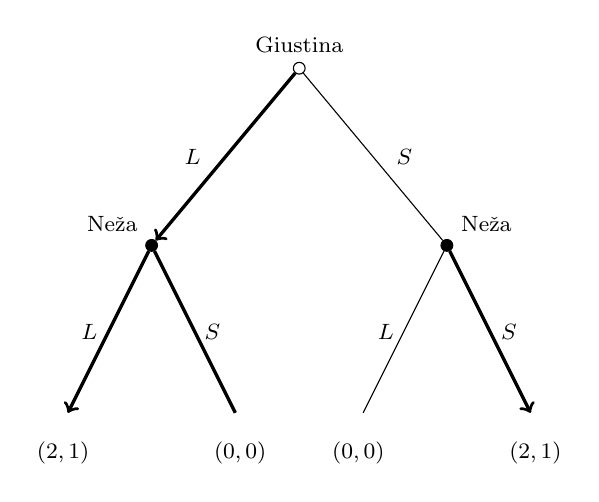
\begin{tikzpicture}[scale=1.5,font=\footnotesize, edge from parent/.style={draw}]
      \tikzstyle{solid node}=[circle,draw,inner sep=1.5,fill=black]
      \tikzstyle{hollow node}=[circle,draw,inner sep=1.5]
      \tikzstyle{level 1}=[level distance=15mm,sibling distance=2.5cm]
      \tikzstyle{level 2}=[level distance=15mm,sibling distance=1.5cm]
      \node(0)[hollow node,label=above:{Giustina}]{}
          child{node(1)[solid node,label=above left:{Ne\v{z}a}]{}
              child{node[label=below:{$(2,1)$}]{} edge from parent[->, very thick] node[left]{$L$}}
              child{node[label=below:{$(0,0)$}]{} edge from parent node[right]{$S$}}
              edge from parent[->, very thick] node[left,xshift=-5]{$L$}
          }
          child{node(2)[solid node,label=above right:{Ne\v{z}a}]{}
              child{node[label=below:{$(0,0)$}]{} edge from parent node[left]{$L$}}
              child{node[label=below:{$(2,1)$}]{} edge from parent[->, very thick] node[right]{$S$}}
              edge from parent node[right,xshift=5]{$S$}
          };
  \end{tikzpicture}\
  SPNE: 
  $\{(L)_G, (L\text{ if L}, S\text{ if S})_N\}$
  \task Normal form w/ underlined BR payoffs: \\
  \begin{tabular}{*{6}{c|}}
      \multicolumn{2}{c}{} & \multicolumn{4}{c}{Ne\v{z}a} \\ \cline{3-6}
      \multicolumn{1}{c}{} &  & $L,L$ & $L,S$ & $S,L$ & $S,S$ \\ \cline{2-6} 
      \multirow{2}*{Giustina}
      & $L$ & \underline{2}, \underline{1} &  \underline{2}, \underline{1} & 0, 0 & 0, 0 \\ \cline{2-6}
      & $S$ & 0, 0 &  1, \underline{2} & 0, 0 & \underline{1}, \underline{2} \\ \cline{2-6} 
  \end{tabular} \\
  $\{(L)_G, (L\text{ if L}, L\text{ if S})_N\}$
  is an NE but not SPNE
  because Ne\v{z}a would be irrational to pick Lion and Owl
  in the off-equilibrium path after Giustina goes to Spice N Steam. \\
  $\{(S)_G, (S\text{ if L}, S\text{ if S})_N\}$
  is another NE that is not sub-game perfect
  because Ne\v{z}a would be irrational to pick Spice N Steam
  in the off-equilibrium path after Giustina goes to Lion and Owl. \\
  \end{tasks}
\end{solution}
\end{question}

\newpage
%------------------------------------------------------------------

\begin{question}%[20]
Consider the strategic form game below:
\begin{table}[!h]
  \begin{center}
    \begin{tabular}{*{6}{c|}}
      \multicolumn{2}{c}{} & \multicolumn{4}{c}{$P_2$} \\ \cline{3-6}
      \multicolumn{1}{c}{} &  & $A$ & $B$ & $C$ & $D$ \\ \cline{2-6} 
      \multirow{4}*{$P_1$}
      & $W$ & 15, -7 &  8,  2 & 18, -7 & 11,  5 \\ \cline{2-6}
      & $X$ & -3, 18 &  6, -7 &  8, -7 & 17, 18 \\ \cline{2-6} 
      & $Y$ &  9, 19 & 20, -4 & 13,  6 & 10, 16 \\ \cline{2-6} 
      & $Z$ & -9, 20 & 14, 16 & 15, -5 & -3,  4 \\ \cline{2-6} 
  \end{tabular}
  \end{center}
\end{table}
\begin{tasks}
  \task 
  Use Iterated Deletion of Strictly Dominated Strategies
  and write out a simplified game table with any remaining cells.
  \task
  Find all Nash equilibria in \textit{pure strategies}.
  Explain why you know they are Nash equilibria.
  % \item 
  % Define mixed strategies for each player
  % using any pure strategies left after IDSDS.
  % Make sure to define all variables you introduce.
  % \item
  % Graph each player's expected utilities as functions of the 
  % other players' mixed strategy you defined in part (c).
  % \item
  % Solve for all Mixed Strategy Nash equilibria in this game.
  % A complete answer will include all calculations used 
  % and a graph of best response functions.
\end{tasks}
\begin{solution}
  \begin{tasks}
    \task
    \begin{enumerate}
      \item $C$ strictly dominated by $A$
      \item $Z$ is now SD by $Y$
      \item $B$ is now SD by $A$
      \item $Y$ is now SD by $W$
      \item no more SD strats, so stop IDSDS
    \end{enumerate}
      \begin{center}
        \begin{tabular}{*{4}{c|}}
          \multicolumn{2}{c}{} & \multicolumn{2}{c}{$P_2$} \\ \cline{3-4}
          \multicolumn{1}{c}{} &     & $A$    & $D$ \\ \cline{2-4}
          \multirow{2}*{$P_1$} & $W$ & \underline{15}, -7 & 11, \underline{5} \\ \cline{2-4}
                               & $X$ & -3, \underline{18} & \underline{17}, \underline{18} \\ \cline{2-4}
        \end{tabular}
      \end{center}
      \task
      NE: $\{X,D\}$ \\
      $X$ is BR to $D$, so $P_1$ has no regrets. \\
      $D$ is BR to $X$, so $P_2$ has no regrets. \\
      neither has any incentive to unilaterally deviate their own strategy.
  \end{tasks}
\end{solution}
\end{question}

\newpage

%------------------------------------------------------------------

\begin{question}
Consider the strategic form game below:
\begin{table}[h!]
  \begin{center}
  \begin{tabular}{*{5}{c|}}
    \multicolumn{2}{c}{} & \multicolumn{3}{c}{Aslanbek} \\\cline{3-5}
    \multicolumn{1}{c}{} & & $Low$ & $Moderate$ & $High$ \\\cline{2-5}
    \multirow{3}*{Hagano}  & $Low$ & 0,0 & 3,2 & 7,3 \\\cline{2-5}
                         & $Moderate$ & 2,3 & 5,5 & 6,4 \\\cline{2-5}
                         & $High$ & 3,7 & 4,6 & 4,5 \\ \cline{2-5}
  \end{tabular}
  \end{center}
\end{table}
\begin{tasks}
  \task
  Find all pure Nash strategy profiles when both play \textit{simultaneously}.
  \task
  Find all pure Nash strategy profiles when \textit{Hagano goes first}.
  Carefully explain all strategy profiles.
\end{tasks}
\begin{solution}
  \begin{tasks}
    \task There are three simultaneous pure strategy NE:
    $\{H_h,L_a\}$, $\{M_h, M_a\}$, and $\{L_h,H_a\}$
    \task 
    There is only one SPNE when Hagano goes first:
    \begin{itemize}
      \item Hagano plays $Low$
      \item Aslanbeck plays:
      \begin{itemize}
        \item $High$ if Hagano plays $High$
        \item $Moderate$ if Hagano plays $Moderate$
        \item $Low$ if Hagano plays $Low$
      \end{itemize}
    \end{itemize}
  \end{tasks}
\end{solution}
\end{question}

\newpage

%------------------------------------------------------------------

\begin{question}
Akua, Barta, and Gilberta are playing a version of hide and seek.
There are only two good hiding spots;
up a tree, or behind a rock.
Akua gets to hide first.
Barta also hides, but she gets to see which spot Akua is hiding
before she picks.
Once Akua and Barta are hidden,
Gilberta has to choose one and only one place to look.
If there are two people hiding in the same spot, 
they crowd each other and Gilberta can see them.
If there is only one person in a spot, Gilberta can't see 
who's hiding there. \\
Create an extensive form game tree
and clearly specify Gilberta's information set.
\begin{solution}
  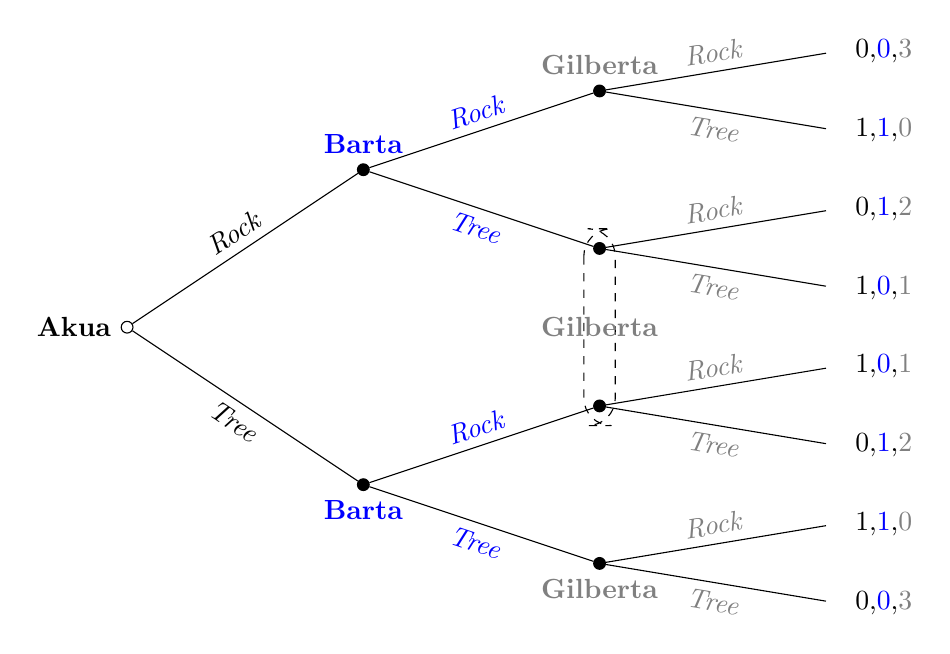
\begin{tikzpicture}[
  grow=right, 
  %edge from parent/.style={draw, very thick},
  level distance = 40mm,
  sibling distance = 25mm,
  %label distance = 1mm
  ]
  \tikzstyle{solid node}=[circle,draw,inner sep=1.5,fill=black]
  \tikzstyle{hollow node}=[circle,draw,inner sep=1.5]
  \tikzstyle{level 1}=[level distance=3cm,sibling distance=4cm]
  \tikzstyle{level 2}=[level distance=3cm,sibling distance=2cm]
  \tikzstyle{level 3}=[level distance=3cm,sibling distance=1cm]
 \node(0)[hollow node, label=left:{\textbf{Akua}}]{}
      child{node(1)[solid node, label=below:{\textbf{\color{blue} Barta}}]{}
          child{node()[solid node, label=below:{\textbf{\color{gray} Gilberta}}]{} 
              child{node[label=right:{0,{\color{blue}0},{\color{gray}3}}]{}
                  edge from parent node[below, sloped]{\textit{\color{gray} Tree}}
              }
              child{node[label=right:{1,{\color{blue}1},{\color{gray}0}}]{}
                  edge from parent node[above, sloped]{\textit{\color{gray} Rock}}
              }
              edge from parent node[below, sloped]{\textit{\color{blue} Tree}}
          }
          child{node(4)[solid node]{}
              child{node[label=right:{0,{\color{blue}1},{\color{gray}2}}]{}
                  edge from parent node[below, sloped]{\textit{\color{gray} Tree}}
              }
              child{node[label=right:{1,{\color{blue}0},{\color{gray}1}}]{}
                  edge from parent node[above, sloped]{\textit{\color{gray} Rock}}
              }
              edge from parent node[above, sloped]{\textit{\color{blue} Rock}}
          }
          edge from parent node[below, sloped]{\textit{Tree}}
      }
      child{node(2)[solid node, label=above:{\textbf{\color{blue} Barta}}]{}
          child{node(3)[solid node]{} 
              child{node[label=right:{1,{\color{blue}0},{\color{gray}1}}]{}
                  edge from parent node[below, sloped]{\textit{\color{gray} Tree}}
              }
              child{node[label=right:{0,{\color{blue}1},{\color{gray}2}}]{}
                  edge from parent node[above, sloped]{\textit{\color{gray} Rock}}
              }
              edge from parent node[below, sloped]{\textit{\color{blue} Tree}}
          }
          child{node()[solid node, label=above:{\textbf{\color{gray} Gilberta}}]{}
              child{node[label=right:{1,{\color{blue}1},{\color{gray}0}}]{}
                  edge from parent node[below, sloped]{\textit{\color{gray} Tree}}
              }
              child{node[label=right:{0,{\color{blue}0},{\color{gray}3}}]{}
                  edge from parent node[above, sloped]{\textit{\color{gray} Rock}}
              }
              edge from parent node[above, sloped]{\textit{\color{blue} Rock}}
          }
          edge from parent node[above, sloped]{\textit{Rock}}
      };
      \draw[dashed,rounded corners=10]($(3) + (-.2,.25)$)rectangle($(4) +(.2,-.25)$);
      \node at($(3)!.5!(4)$){\textbf{\color{gray} Gilberta}};
  \end{tikzpicture} \\
  \underline{Gilberta's information set:}
  \begin{itemize}
    \item Either both players are behind the Tree,
    \item or both players are behind the Rock,
    \item or: either Akua is behind the Rock and Bartua is behind the Tree;
    or Akua is behind the Tree and Bartua is behind the Rock
    (represented on the tree by the circled nodes)
  \end{itemize}
\end{solution}
\end{question}

\newpage

%------------------------------------------------------------------

\begin{question}
Suppose that two fishing boats are selling to the same market.
Let $V$ be the tons of fish caught by Vlatislav's boat,
and $J$ be the tons of fish caught by Jeren's boat.
People in this town only want to buy so many fish,
so the price $P$ of fish is given by the inverse demand function:
  $$P = 60 - (V+J)$$
Assume that Vlatislav has a marginal cost of 30
and Jeren has a marginal cost of 36.
\begin{tasks}
  \task Solve for Vlatislav's best response rule
  as a function of $J$.
  \task Solve for Jeren's best response rule
  as a function of $K$.
  \task
  Graph both players' best response functions 
  and find all Nash Equilibria.
  Label your graph appropriately.
\end{tasks}
\begin{solution}
  \begin{tasks}
    \task
    \begin{align*}
      \Pi_v & = (60 - V - J)V - 30 V \\
            & = 60V - V^2 - VJ - 30 V \\
      \frac{d\Pi_v}{dV} & = 60 - 2V - J - 30 \\
      BR_V(J) & = \frac{60-30-J}{2} = 15 - \frac{J}{2}
    \end{align*}
  \task
  \begin{align*}
      \Pi_j & = (60 - V - J)J - 36 J \\
      \frac{d\Pi_j}{dJ} & = 60 - 2J - V - 36 \\
      BR_V(J) & = \frac{60-36-V}{2} = 12 - \frac{V}{2}
  \end{align*}
  \task
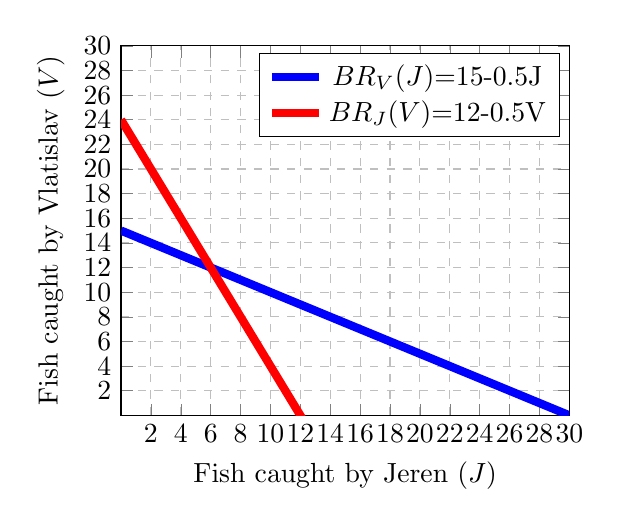
\begin{tikzpicture}
  \begin{axis}[
    width=0.6\textwidth,
    grid,
    ylabel={Fish caught by Vlatislav ($V$)},
    xlabel={Fish caught by Jeren ($J$)},
    xmin=0, xmax=30,
    ymin=0, ymax=30,
    xtick={2,4,...,30},
    ytick={2,4,...,30},
    grid style=dashed,
    ]
    \addplot [
        domain=0:30,
        line width=3pt,
        color=blue,
        ] 
        {15-0.5*x};
        \addlegendentry{\(BR_V(J)\)=15-0.5J}
        \addplot [
        domain=0:30,
        line width=3pt,
        color=red,
        ] 
        {24-2*x};
        \addlegendentry{\(BR_J(V)\)=12-0.5V}
    \addplot[draw=none] coordinates {(1,1)};
  \end{axis}
\end{tikzpicture} \\
\underline{NE:} $(J=6, J=12)$ is the only strategy profile
where both players' best responses intersect.
  \end{tasks}
\end{solution}
\end{question}
%------------------------------------------------------------------

\end{document}
